%% Example document for the eis_msc_thesis document class. Compile with
%% pdfLaTeX or LaTeX.
%%
%% Created: April 7, 2004, by Johan Carlson
%% Last modified: June 7, 2009, by Johan Carlson


%% Pick one of the following depending on the language of the report, and if 
%% you want twosided or onesided print.
%% Also change language definition after \begin{document}

% English, twosided

\documentclass[12pt,a4paper,openright,final,twoside,en]{csee_msc_thesis} 

% English, onesided    
%\documentclass[12pt,a4paper,openright,final,oneside,en]{csee_msc_thesis}     

% Swedish, twosided
%\documentclass[12pt,a4paper,openright,final,twoside,sv]{csee_msc_thesis}     

% Swedish, onesided
%\documentclass[12pt,a4paper,openright,final,oneside,sv]{csee_msc_thesis}     

%%==================================================================
%% Class options specific to this class
%%==================================================================
%%   en, sv  - Swedish or English
%%   parskip - Use blank row instead of indentation for
%%             new paragraphs
%%==================================================================

%% These packages are not required in general,
%% only for some examples in this document.
\usepackage{fancybox}
\usepackage{verbatim}
\usepackage{listings}
\begin{document}

%%==================================================================
%% Define variables here
%%==================================================================

\def\thesistitle{An Example Master's Thesis}
\def\theauthor{Johan E.\ Carlson}
\def\theaddress{Lule� University of Technology\\
            Dept.\ of Computer Science and Electrical Engineering\\
            Div.\ of Systems and Interaction}

% Define the English abstract
\def\theabstract{ProMoVis provides an environment where engineers may, through a combination of graphical visualisation and powerful analysis tools, analyse and deepen their understanding of complex processes and its components. Currently a drawback is that the user has to create a model of the system, through the graphical interface that ProMoVis provides, even though he may have existing models created in another environment.\\\newline This report describes the design process and implementation of a tool, written in python, that utilizes the JModelica environment to export models, described in Modelica, to an equivalent SFG representation used in ProMoVis. This is done through linearising a model around an operating point and then extracting a DAE representation of it. From this DAE, it is then possible to extract an SFG representation, describing how a component depends on other components in the system.\\\newline Besides demonstrating the key algorithm for extracting the SFGs this report also discusses the design of the software and how the internals of the tool is divided into separate phases. Phases responsible for compiling the original model, building an intermediate representation of the SFGs for internal use, validation of the system together with some optional transformations of the original model and finally the actual generation of the ProMoVis representation from the intermediate representation. }
\def\thepreface{I worked on this project during the spring of 2012 starting out as a novice in the field of control theory and physical modeling with only the most fundamental knowledge in the subject. But having been in touch with Modelica in earlier courses, and found it to be a powerful tool that I would like to deepen my understanding of. It was not hard to accept when Wolfgang Birk proposed this project.\\\newline The source code to the tool is currently available at https://github.com/jwmbrg/Modelica-to-PromoVis-export, although I probably will move the actual export software to a separate repository, without the school related information, for continued development after this project has ended.\\\newline I would like to thank Wolfgang Birk and Miguel Casta{\~{n}}o for the time and effort they have put down,  with their pragmatic approach, they have been invaluable in giving me a deepened understanding of the field of control theory and mathematical modeling.\\\newline Finally, I would like to give credit to Johan Carlson for providing the \LaTeX{} template used in formatting this report. \\\newline Hopefully the output of the project, the export tool, might help make ProMoVis more accessible to existing users of Modelica and also provide a foundation for a tighter integration between the two environments.\\\newline
\vspace*{2cm}%
\hfill Jesper Moberg
}
\def\thedate{Template version: \theclassversion , \theclassdate}

% Use this if you want a Swedish abstract
%\def\theswedishabstract{\input{SweAbstract/sweabstract.tex}}

%%==================================================================
%% Generate preamble pages here (This should not need any changes)
%%==================================================================
\startpreamble
  {\thesistitle}
  {\theauthor}
  {\theaddress}
  {\theabstract}
  {\thepreface}
  {\thedate}
 % {\theswedishabstract} % use this for Swedish abstract, leave empty for English

%%==================================================================
%% Start including the chapters
%%==================================================================
% First argument is the "running titles", second is the chapter name.
\makechapter{Introduction}{Introduction\label{ch1}}
\section{Background}
%During a research project at LTU a tool was developed, called ProMoVis,  aimed at structure analysis and visualisation of complex physical processes.
While Modelica, Simulink and other existing tools are very powerful when it comes to simulation and modelling of  dynamic systems there is a need for a tool that can aid engineers in selecting different control structures by making it possible to analyse specific interconnections in dynamic systems. %A drawback with existing tools is that although a user declares the relations between inputs and outputs, at simulation time the models are still assumed to be treated as "black boxes". Making it hard to monitor and analyse the internal behaviour of components in the modelled systems. 
Due to the identified need for a tool that can solve these problems \cite{ProMoVisPaper}\nocite{*}, the design and implementation of ProMoVis started in 2010 which recently was released as an open source project.
\section{Problem Description}
As stated earlier, ProMoVis purpose is visualisation and analysis of large systems. It assumes that the user has information about the components of the system and the relations between them.  Today, %there is no scripting interface to ProMoVis and 
models have to be created in the graphical environment by placing the components and defining the relations one by one. This is a task that can become very tedious and error-prone for many systems. At the same time a user that would benefit from using ProMoVis in his design process can be assumed to already have existing models, from another environment, available. Therefore the possibility to import existing models would make ProMoVis more accessible to its intended users.
\section{Project Goal}
In recent time Modelica, as a tool for modeling of physical systems, has shown an increase in popularity and has become somewhat of a standard for describing physical systems. Due to its widespread use and the amount of open source tools that are available for models described with help from the language, this projects goal is to implement a tool that can import models, described in Modelica, into ProMoVis. This tool should try to preserve as much information and semantics from the original Modelica models but, at the same time, keep the effort needed from the user to perform the export at a minimum. A final demand is that the tool should be easy to integrate with the existing ProMoVis environment so that imports can be performed from within ProMoVis.
% Features needed
%There is a need to a tool for control structure selection. It should analyse the interconnections in a dynamic system and how a control strategy should be shaped. This very different from what you write here.]





\makechapter{Theory}{Theory\label{ch2}}
\section{Workflow}
During the projects initial phase much of the time was put on familiarizing with the ProMoVis and JModelica enviroments and the math that acts as a foundation for the Modelica models. During these first weeks there were sporadic meetings and discussions with the supervisor whenever problems or questions appeared. After an initial meeting with the developer of the ProMoVis frontend (See Appendix \ref{appC}). The start of the development of a first "Proof of concept" was initiated. After finishing this, a more thorough design phase started where both the developers of ProMoVis and a "test-user" got involved in the process. 
\section{Tools}
\subsection{Modelica}
Modelica is a object-oriented declarative programming language used to create models of physical system. Unlike many other modelling languages, Modelica is not domain specific and thus can be used to model physical systems consisting of a mix of electrical, mechanical and chemical processes. Since the release of the first language specification in 1997 the continuous development of the language has been maintained by the Modelica Association and the current version of the Language specification is 3.2 \cite{ModelicaSpec}.\nocite{*}
\subsection{JModelica}
There is several environments, both proprietary and open source, that provides tools for compilation, analysis and simulation of  models described in Modelica. Since the use of proprietary software would demand that we separate the export tool from ProMoVis. An initial demand on the environment to be used was that it should be open source. After examining the options available JModelica\cite{jmodelicaorg}\nocite{*} was choosen because of its Python front-end, that makes it easy to interface with the tool from other software while still providing a structured environment around which we can build all parts of the export tool.   
\subsection{Numpy and SciPy}
Another important feature supporting the use of the JModelica platform was its tight integration with the NumPy and SciPy packages \cite{scipyorg}\nocite{*}. These are two very popular open source packages for Python providing a strong and well documented toolbox for mathematical computing. When extracting the mathematical models through JModelica they are represented using the data-structures provided by NumPy and in many cases this removes the need to "reinvent the wheel" for many of the operations that needs to be performed on the mathematical models before export. Instead one can directly use existing methods provided by SciPy and NumPy. The use of this package also makes the source-code for the export tool more accesible to other programmers familiar with Python and these packages.
\subsection{The SFG}
Since the SFG is a fundamental concept in ProMoVis it is motivated to give a brief introduction to how it is used in ProMoVis. ProMoVis bases its analysis and visualisation on SFG representations of dynamical systems. It is this representation the tool needs to be able to accurately extract from the existing Modelica models. Basically the an SFG is a directed graph with the vertices representing each of the states in the systems and the edges representing the relation, in terms of transfer functions, between the vertices.\\\newline The simple two tank system in Fig.~\ref{fig:twotank} Can be described by the general equations.

\begin{figure}

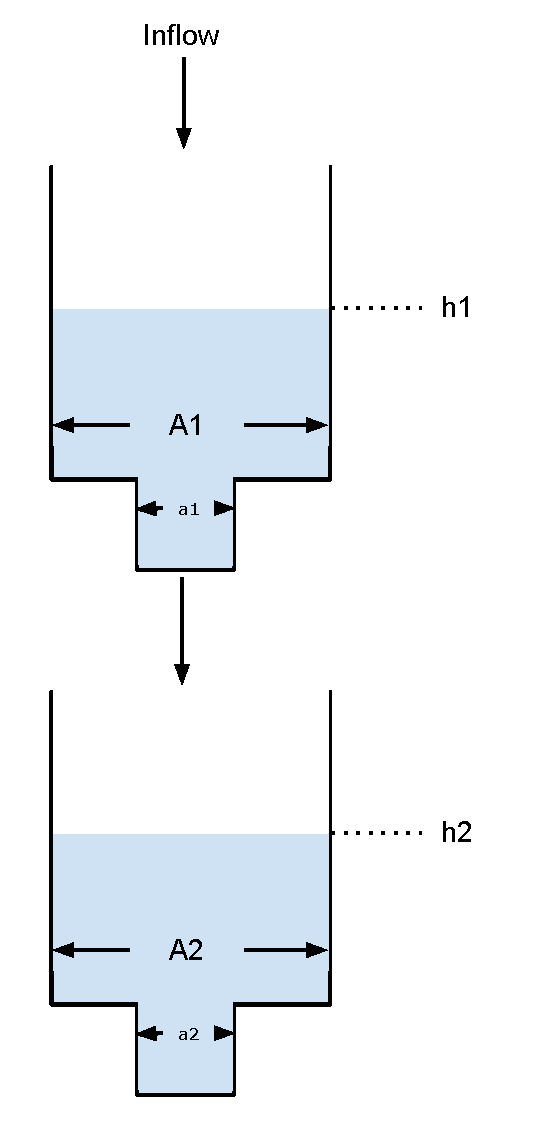
\includegraphics[scale=0.4,bb=0 0 3.67in 7.47in] {Figures/TwoTankSystem.pdf}\\\newline
\caption{A simple two tank system}
\label{fig:twotank}
\end{figure}
\begin{equation}
    \dot{h_1} = -a_1/A_1*\sqrt{2*g*h_1} + inflow\\\newline
\end{equation}
\begin{equation}
	\dot{h_2} = -a_2/A_2*\sqrt{2*g*h_2} + a_1/A_1*\sqrt{2*g*h_1}
\end{equation}
Linearising the specific model, described in Modelica,  in Appendix \ref{appD}. We can then extract the transfer functions. For the parameters specified the following is obtained:\\\newline
Transfer function from inflow to h1 is : $\begin{array}{rcl} \frac{1}{s +2.3*10^{-2}} \end{array}$\\\newline
Transfer function from h1 to h2 is :$\begin{array}{rcl} \frac{2.3*10^{-2}}{s +8.9*10^{-2}} \end{array}$\\\newline
And the corresponding signal flow graph, as shown in Fig.~\ref{fig:sfg}, can be obtained. From the figure, it is easy to see that the vertices in the SFG is the states of the system and the edges are the transfer functions between the states. In ProMoVis, there is also additional information supplied with the vertices, such as operating point, saturation values etc. 
\begin{figure}
\fbox{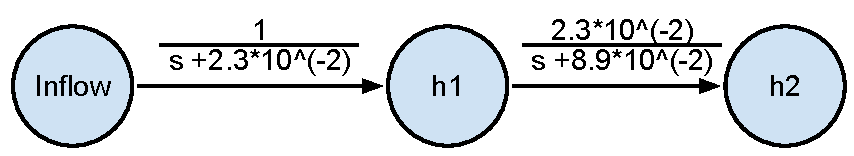
\includegraphics[scale=0.8,bb=0 0 5.69in 1.04in] {Figures/sfgtwotank.pdf}}
\caption{Corresponding SFG for the two tank system in Fig~\ref{fig:twotank}}
\label{fig:sfg}
\end{figure}


\makechapter{Method}{Method\label{ch3}}
To add a second chapter, simply include it in the main document.

\section{General structure}
\subsection{JModelica(Compile)Phase}
The JModelica environment is used to compile the Modelica models to JModelicas JMU representation \cite{jmodelicaorg}\nocite{*}. This representation is internally represented as a, possibly nonlinear, DAE. Since ProMoVis assumes the systems to be linear, the compiled model needs to be linearised around an operating point. Here an assumption is made, that the model is stable at Time 0.\\\\After linearisation a DAE on the following form can be extracted:
\begin{equation}
E*dx = A*x + B*u + F*w + g
\end{equation}
This represenation should be familiar, the x and dx vectors represents the states and outputs of the linearized system. The u vector represents declared inputs, w is algebraic varibles, that is all variables in the system that has no derivative declared.Finally g is a constant bias.\\\\The linearization also outputs some useful information that we later use in the generation of ProMoVis scenarios:
\begin{itemize}
\item \textit{State names}, corresponding to the declared variable names from the original Modelica file.
\item \textit{Input names}, corresponding to the declared input names from the original Modelica file.
\item \textit{Algebraic names}, corresponding to the declared algebraic variable names from the original Modelica file.
\item \textit{Operating points} for the linear model \textit{dx0},\textit{w0}, \textit{u0} and \textit{x0}. Which is , in later stages, used to provide feedback for the user regarding the validity of the resulting model.
\end{itemize}
From now on we will refer to states and algebraic variables as simply "variables" and whenever a distinction between the two is needed, it will be explicitly declared. 

\subsection{Generation of the internal structure}
When the DAE is obtained, the task is then to extract the relations between the variables from it. Here we choose to collect and store each of the variables, together with each of the variables that acts as input to it. It might feel more natural to store a variable together with each of its outputvariables but since ProMoVis supports both conventions and due to the fact that it is straight forward to solve a variable for all its inputs from the original DAE the first representation was choosen.
The generation of the internal structure is best illustrated with the following example.\\\newline
If we assume two state variables and two algebraic variables, the general structure of the DAE would look like the following:\\\newline
$
\begin{bmatrix} E_{11} & E_{12} \\ E_{21} & E_{22} \\ E_{31} & E_{32} \\ E_{41} & E_{42} \end{bmatrix} \left[ \begin{array}{c} x0' \\ x1' \end{array} \right]
= \begin{bmatrix} A_{11} & A_{12} \\ A_{21} & A_{22} \\ A_{31} & A_{32} \\ A_{41} & A_{42} \end{bmatrix} \times \left[ \begin{array}{c} x0 \\ x1 \end{array} \right] + \begin{bmatrix} B_{11} & B_{12} \\ B_{21} & B_{22} \\ B_{31} & B_{32} \\ B_{41} & B_{42} \end{bmatrix} \times \left[ \begin{array}{c} u0 \\ u1 \end{array} \right]+
\begin{bmatrix} F_{11} & F_{12} \\ F_{21} & F_{22} \\ F_{31} & F_{32} \\ F_{41} & F_{42}\end{bmatrix} \times \left[ \begin{array}{c} w0 \\ w1 \end{array} \right]$

The task is now, to find which of the rows in the system that should be solved for which variable so that the whole system can be solved. A demand on the system is that it should not contain any Algebraic loops. For a more thorough discussion regarding this please review Appendix \ref{appA}\\\\After retrieving which row that we should solve for which of the variables we build up an intermediate representation of the SFG where we store each of the variables together with all of its input variables. Where input variables are the states and algebraic variables that directly affect the variable we solve for.\\\\
As an example, if we assume that we should solve row 1 for x0 the procedure is as follows:\\\\$\begin{array}{rcl} E_{11}*x0*s  +E_{12}*x1*s=A_{11}*x0  +A_{12}*x1 +B_{11}*u0  +B_{12}*u1  +F_{11}*w0  +F_{12}*w1 \end{array}$\\
\\Putting x0 alone on the left-hand side and collecting the coefficients then yields:\\\\$\begin{array}{rcl} (E_{11}*s-A_{11})*x0  =(A_{12}-E_{12}*s)*x1 +B_{11}*u0  +B_{12}*u1 +F_{11}*w0  +F_{12}*w1 \end{array}$\\\\
Finally, solving for x0 yields:\\\\
$\begin{array}{rcl} x0  = \frac{(A_{12}-E_{12}*s)}{(E_{11}*s-A_{11})}*x1 +\frac{B_{11}}{(E_{11}*s-A_{11})}*u0  +\frac{B_{12}}{(E_{11}*s-A_{11})}*u1 ++\frac{F_{11}}{(E_{11}*s-A_{11})}*w0 +\frac{F_{12}}{(E_{11}*s-A_{11})}*w1\end{array}$\\\newline Which would correspond to the following SFG:\\Internally we then represent each of the variables in the following form.\\\newline
%

\setlength\fboxsep{0pt}
\setlength\fboxrule{0.5pt}
\fbox{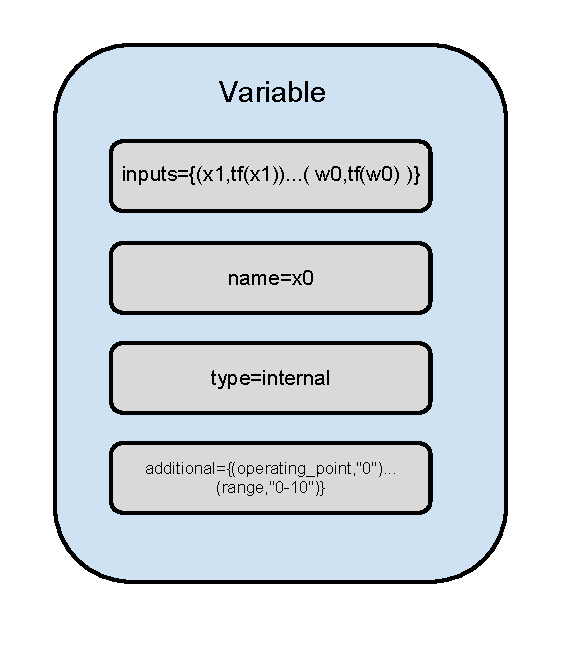
\includegraphics[scale=0.8,bb=0 0 97mm 111mm] {Figures/variable_structure.pdf}}\\\newline Here "inputs" is a dictionary with variable names as keys and the corresponding transfer functions as a values. A transfer function, in the export tool,is using the same convention as in MatLab to represent the numerator and denominator coefficients for a transfer function in two separate arrays. It also has some methods, described later, that are used in the generations of the ProMoVis specific structure. 


\subsection{Validation and Transformations}
Wh
\subsection{Scenario generation}
When the structure is validated and all optional transformations are done. The actual generation of the ProMoVis represenation is straight forward. Basically the ProMoVis representation contains two parts. First the descriptive part, a collection of all variables, with their names, graphical layout and additional mathematical properties. The second part,  the processmodels, describes the relation between a variable and the other variables in the system. 
\subsubsection{Graphical Layout}
Even though Modelica supports description of position and graphical represenation of models through its annotations interface, these are not necessary for a valid Modelica model. Therefore no effort has been put into trying to recieve this type of meta-information. Instead, to make sure that a user of ProMoVis is able to easilly access and attach controllers to the generated model the variables are emitted as depicted in the figure below.\\\newline
\setlength\fboxsep{0pt}
\setlength\fboxrule{0.5pt}
\fbox{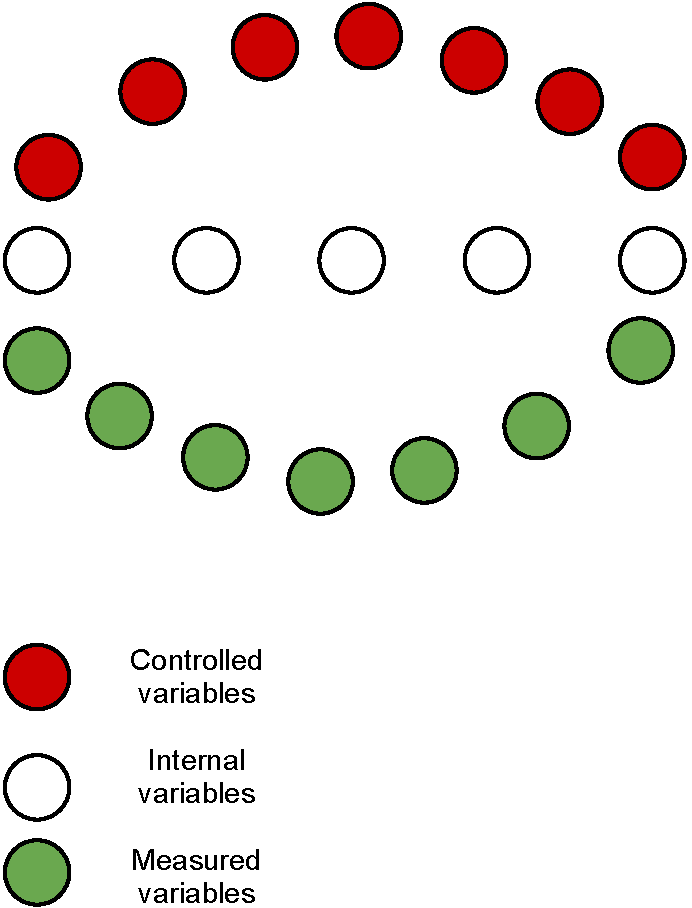
\includegraphics[scale=0.8,bb=0 0 117mm 154mm] {Figures/layout.pdf}}\\\newline

That is, inputs and measured variables are emitted as the upper and lower half of a circle while internal variables, that are assumed to not be of interest, are collected in the center of the circle. This achieved by a helper object, the layout emitter, that is initiated with the number of internal, measured and input variables and then calculates the step size in x and y direction that will eventually achieve the circular shape. 

When we then iterate over each of the variables to get their corresponding descriptive part, the layout emitter is passed as an argument, so that it can be queried for the variables graphical x and y position. This i done in a very naive way, the layout emitter has counters for each of the variable types and then, each time it is queried, it increments the current counter value together with the previously calculated step sizes to generate one x,y coordinate that is returned to the querying variable. 
\subsubsection{Additional information added}

\section{Interfacing with the tool}
Since there are several seperate phases in the tool, and each of the phases might later be extended with additional options and necessary parameters xml is used to pass information to the tool. By using xml and not command line arguments one might, through using existing modules for xml-parsing and object representation of the xml files, just pass the instance of the "parsed" xml document to each of the phases. Where they then might extract the information needed for the phases.FIXME\\\\Following is an example of the input file to the tool, containing all the necessary parameters.
\begin{lstlisting}
<?xml version="1.0" ?> 
<root>
        <filepath>C:\Users\Public\Documents\QuadTankPack.mo</filepath>
        <model>QuadTankPack.QuadTank</model>
        <mpattern>_pmv;_fooBar;x2</mpattern>
        <outputpath>C:\ProMoVis\output.xml</outputpath>
        <pmvoutputpath>C:\ProMoVis\QuadTank.pmv</pmvoutputpath>
</root>
\end{lstlisting}
The filepath and model nodes are the path to the original modelica source file and the full model name, including packagenames, of the target model. The node, mpattern, contains regular expression that the tool will try to match the ending of variable names on, so that if it encounters the variables foo\_pmv, foo\_foobar, foox2 or x2 it will make sure that those variables are indicated as measured variables in the ProMoVis representation.


\section{DAE vs ODE}
Readers familiar with Modelica and the JModelica environment might be accustomed to working on the ODE-representation of systems. The reason that we stick with the DAE even though the extraction of the SFG from the ODE is less complex is due to the fact that when using the ODE we loose casuality whenever an algebraic variable is in a path. For a more thorough dicussion see Appendix \ref{appB}.




\makechapter{Implementation}{Implementation\label{ch4}}
\section{A small example}
In this chapter a small Modelica model is compiled, translated and exported to ProMoVis through the export-tool. The files used are available, together with the source code, at GitHub\cite{githabb}\nocite{*}.

\subsection{The input model}

The model used for the example:
\lstset{language=modelica}
\begin{lstlisting}
package QuadTankPack
  model QuadTank
    // Process parameters
	parameter Modelica.SIunits.Area A1=4.9e-4, 
									A2=4.9e-4, 
									A3=4.9e-4, 
									A4=4.9e-4;
	parameter Modelica.SIunits.Area a1(min=1e-6)=0.03e-4, 
									a2=0.03e-4, 
									a3=0.03e-4, 
									a4=0.03e-4;
	parameter Modelica.SIunits.Acceleration g=9.81;
	
	parameter Real 	k1_nmp(unit="m^3/s/V") = 0.56e-6, 
					k2_nmp(unit="m^3/s/V") = 0.56e-6;
	parameter Real g1_nmp=0.30, g2_nmp=0.30;

    // Initial tank levels
	parameter Modelica.SIunits.Length x1_pmv_0 = 0.04102638;
	parameter Modelica.SIunits.Length x2_0 = 0.06607553;
	parameter Modelica.SIunits.Length x3_0 = 0.00393984;
	parameter Modelica.SIunits.Length x4_foo_0 = 0.00556818;
	
    // Tank levels
	Modelica.SIunits.Length x1_pmv(start=x1_pmv_0,min=0.0001);
	Modelica.SIunits.Length x2(start=x2_0,min=0.0001);
	Modelica.SIunits.Length x3(start=x3_0,min=0.0001);
	Modelica.SIunits.Length x4_foo(start=x4_foo_0,min=0.0001);
	Real x1plusx2(start=0);
	// Inputs
	input Modelica.SIunits.Voltage u1;
	input Modelica.SIunits.Voltage u2;

  equation    
    der(x1_pmv) = 	-a1/A1*sqrt(2*g*x1_pmv) + a3/A1*sqrt(2*g*x3) 
					+ g1_nmp*k1_nmp/A1*u1;						
	der(x2) 	= 	-a2/A2*sqrt(2*g*x2) + a4/A2*sqrt(2*g*x4_foo)
					+ g2_nmp*k2_nmp/A2*u2;
	x1plusx2	=	x2+x1_pmv;
	der(x3) 	= 	-a3/A3*sqrt(2*g*x3) 
					+ (1-g2_nmp)*k2_nmp/A3*u2;
	der(x4_foo) = 	-a4/A4*sqrt(2*g*x4_foo) 
					+ (1-g1_nmp)*k1_nmp/A4*u1;

  end QuadTank;
end QuadTankPack;
\end{lstlisting}
This is basically the same model as provided in the JModelica examples with some small changes. The initial values have been configured in such a way that the system is at equilibrium at time zero. As stated earlier, this is something the user has to verify beforehand with the help of the Modelica environment used. Besides the initial values a variable, x1plusx2, have been added to the model. This is done entirely to introduce an algebraic variable in the system.
\subsection{Running the export}
After setup of the input file as depicted in chapter 3, indicating that variables with "\_pmv", "foo\_" and "x2" should be set as measured variables, the exporttool is called. After checking that no warnings were generated, the result can be viewed in ProMoVis:
\setlength\fboxsep{0pt}
\setlength\fboxrule{0.5pt}
\fbox{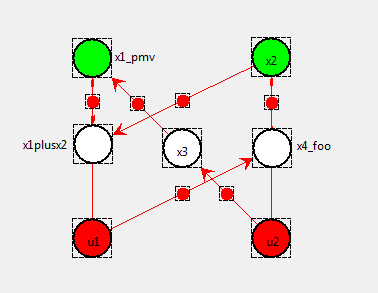
\includegraphics{Figures/exportSFG.png}}\\\newline
As seen,  x1\_pmv and x2 has been set as measured variables, matching with \_pmv and x2 respectively, while none of the variables matched with the pattern "foo\_". If we start by inspecting the process model for x1plusx2:\\\newline
\setlength\fboxsep{0pt}
\setlength\fboxrule{0.5pt}
\fbox{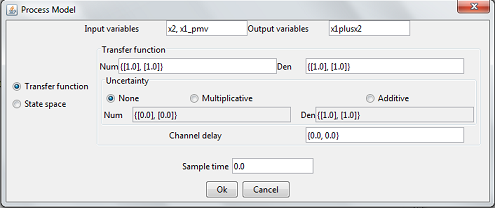
\includegraphics{Figures/x1plusx2Rel.png}}\\\newline
Here, due to the fact that all the variables are represented as Multiple input, single output process models, it doesn't matter which of the incoming arrows to x1plusx2 that is examined. All of the inputs, as depicted in the dialogue, are displayed. As expected, the transfer functions is unity, for both of the input variables to x1plusx2. \\\newline
Examining the properties of the variable yields:

\setlength\fboxsep{0pt}
\setlength\fboxrule{0.5pt}
\fbox{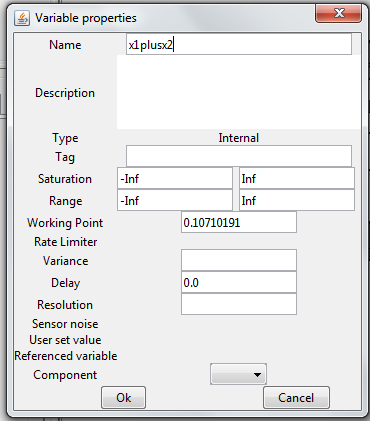
\includegraphics{Figures/x1plusx2OPP.png}}\\\newline
Since the initial values for x1\_pmv and x2 were set in the original model, the working(operating) point of x1plusx2 is the sum of the initial values.\\\newline
Lets look at a variable with some more complex input relations. Choosing x2 it should have both x4\_foo and u2 as inputs and contain a derivative.\\\newline
\setlength\fboxsep{0pt}
\setlength\fboxrule{0.5pt}
\fbox{\includegraphics{Figures/x2rel.png}}\\\newline
From the picture we can see that the input relations are:\\
$\begin{array}{rcl} \frac{-3.4285E-4}{-s -0.05275}*u2 \end{array}$\\
$\begin{array}{rcl} \frac{-0.1817}{-s -0.05275}*x4\_foo \end{array}$\\\newline
Looking at the denominators, they are both the same, recalling the algorithm, described in Appendix \ref{appA}, one can see that this will always be the case for all of the inputs to a variable, they will all share a common denominator.

\makechapter{Discussion}{Discussion\label{ch5}}
To add a second chapter, simply include it in the main document.

\section{Discussion}
\subsection{Limitations}


\subsubsection{Conditional values}
A thing that should be implemented is the ability to extract min, max, nominal and other additional parameters that a variable may have in a Modelica-model since this information would also be useful in a generated ProMoVis-representation. But right now there does not seem to be a way to extract this through JModelica. A forum post has been created, at jmodelica.org, regarding the absence of this possibility.
\subsubsection{The graphical representation}
Although the translation between Modelica and the ProMoVis-representation is now possible, the two environments is not integrated with each others in such a way that one can do modifications in Modelica, and then only the affected parts of the system is changed in ProMoVis. This is a significant drawback when it comes to the visualisation purpose of ProMoVis. A user that has imported a Modelica model into ProMoVis and done some custom layout and maybe added additional graphical representation through ProMoVis components, cant reuse this information when re-running an export, even though he might only have changed the operating points of the Modelica model.\\\newline There exists two general approaches to this problem: 
\begin{itemize}
\item One could add the possibility to do the export with a former ProMoVis-file as additional input. Then let the export tool could scan through the old file, look for variables with the same name and re-use the graphical information from that node. This approach still demands that the user add the graphical information needed for visualisation after the first export.
\item Another approach is to add support for extracting information from graphical annotations. The graphical annotations are a standardised, through the specification of the language \cite{ModelicaSpec}\nocite{*}, way of creating a visual representation of a modeled system and its components.
\end{itemize}Of this two approaches, the later should be the one to aim for since supporting the interpretation of graphical annotations in the export-tool could make the transition between a users Modelica environment and ProMoVis a one-click effort. 

\section{The goal}
This project has shown that it is indeed possible to extract and translate models from Modelica into ProMoVis but for future development the challenge does not lie in any issues related to control theory or mathematical obstructions FIXME. Instead, the challenge lies in making it convenient for the user. 


%%==================================================================
%% Include any appendices here.
%%==================================================================
\appendix % This command initializes the appendix part, Don't change!

%% Include appendix A, add more if needed
\makeappendix{Appendix A}{Least squares fit of response surface
models by multiple linear regression\label{appA}}

\section{Deciding which variable to solve first}
When extracting the SFGs from the DAE one has to make sure that one solves each of the rows for the correct variables making sure that you can extract an SFG for every variable in the system.Recall the general equation for the DAE:
\begin{equation}
E*dx = A*x + B*u + F*w + g
\end{equation}
If no algebraic equations are present in the orignal Modelica model, the resulting DAE would have the following form:
\begin{equation}
E*dx = A*x + B*u + g
\end{equation}
The number of rows in such a system, containing no algebraic variables, would be the same as the amount of the number of declared or inferred states in the systems. The introduction of algebraic variables, that we recall are all variables that does not have a declared derivative, adds 1 row to the DAE.Since states, by definition, has a derivative declared, we can therefore look only at the E and F matrices to solve the problem of which row to solve for which variable. Since a state has to be solved for a row containing its derivative. If we declare:
\begin{equation}
S=[E|F]
\end{equation}
Here we easilly realize that the S matrix will be an nxn matrix, since we by concatenating the E and F matrix, add as many columns that there is extra rows.\\
With the column vector L
\begin{equation}
L=[dx_0...dx_i, w_0...w_i]
\end{equation}
We then examine this system:
\begin{equation}
S*L
\end{equation}
By examining each of the columns in S and storing all the rownumbers that contains non-zero elements together with the variable corresponding to the column a list is retrieved for each of the variables.This  list i containing all the rownumbers where the variable is present.
The pseudocode for this process might look something like this:
\begin{lstlisting}
varDict.initWithKeysAndValues(L,[])
for row in S {
	for col in row{
		if(col.value !=0){
			key=L(numberOf(col));
			value=numberOf(row)
			list=varDict(key)
			list.append(value)		
		}
	}			
}
\end{lstlisting}
As one can see, this approach has a quadratic running time, no matter the input, compared to a pure gaussian elimination approach, that has a cubic time complexity.

The task is then to start extracting the SFGs from the original DAE with the help of this list. If the system contains no algebraic loops, it should be possible to iterate through the dictionary and find a variable that has only one rownumber associated with it. Removing that variable from the dictionary and remove the corresponding rownumber from the remaining variables in the dictionary.

Pseudocode for this process:
\begin{lstlisting}
int i=0
int looped=0 // looped is used to detect algebraic loops
solvList=[]
while(varDict!=empty && looped !=2) {
	key=varDict(i).key
	list=varDict(key)
	if(lengthOf(list)==1){
		//add a tuple with rownumber and key
		rowNumber=list[0]
		solvList.append((key,rowNumber);
		//remove the key (variable), since the
		// problem is solved for this key
		varDict.remove(key)
		
		for otherLists in varDict{
			//we remove the rownumber 
			//from the rest of the variables.
			//Since this row is already consumed
			//in the solution
			otherLists.remove(rowNumber)
		}
		looped=0; 	//If we solved for a variable, 
					//reset looped.
	}
	i=i+1;
	if(i>varDict.size()){
		i=0; //restart the process from the beginning
		looped+=1; // increment looped 	
	}			
}
if(looped==2){
	print "failed due to algebraic loops
}else{
	print "success"
}

\end{lstlisting}

At this point, we have a list of tuples, with each of the tuples containing a variable name and a row number, and we can begin to extract the SFGs from the DAE by solving each of the variable for the given rownumber.
\makeappendix{Appendix A}{Solving DAE-system in correct order\label{appB}}
Recall the general DAE representation:
\begin{equation}
E\dot{x} = Ax + Bu + Fw + g
\end{equation}Introducing the ODE representation that also can be extracted:
\begin{equation}
\dot{x} = Ax + Bu + g
\end{equation}
\begin{equation}
w  = Hx + Mu + q
\end{equation} Here it might be tempting to create the SFGs from the ODE instead, since one can extract the SFGs  for the states and algebraic variables separately. But notice, now the states does not depend at all on the algebraic variables in w. This is still a correct system, since algebraic variables is only a combination of states,other algebraic variables and constants thus can be reduced and replaced by other states and a constant. But even though it is mathematically correct, we have lost information. The causality is broken, and a user that has declared states that depends on algebraic variables can no longer view and analyse such relations inside ProMoVis. If we consider the fictional, system:

\begin{equation}
\dot{x_1}=x_2+w_1+u_2
\end{equation}
\begin{equation}
\dot{x_2}=x_3+u_1
\end{equation}
\begin{equation}
\dot{x_3}=x_1
\end{equation}
\begin{equation}
w_1=x_3+x_2
\end{equation}The DAE representation of the system is then:
\begin{equation}
\begin{bmatrix}  1 & 0 & 0 \\ 0 & 1 & 0  \\ 0 & 0 & 1 \\ 0 & 0 & 0   \end{bmatrix}  \left[ \begin{array}{c} \dot{x_1} \\ \dot{x_2} \\ \dot{x_3} \end{array} \right]
= \begin{bmatrix} 0 & 1 & 0 \\ 0 & 0 & 1 \\ 1 & 0 & 0 \\ 0 & 1 & 1 \end{bmatrix}  \left[ \begin{array}{c} x_1 \\ x_2 \\ x_3 \end{array} \right] + \begin{bmatrix} 0 & 1 \\ 1 & 0 \\ 0 & 0 \\ 0 & 0 \end{bmatrix} \left[ \begin{array}{c} u_1 \\ u_2 \end{array} \right]+
\begin{bmatrix} 1 \\ 0 \\ 0  \\ -1 \end{bmatrix} \left[ \begin{array}{c} w_1 \end{array} \right]
\label{fig:eqDAE}
\end{equation}
%
\begin{figure}
\fbox{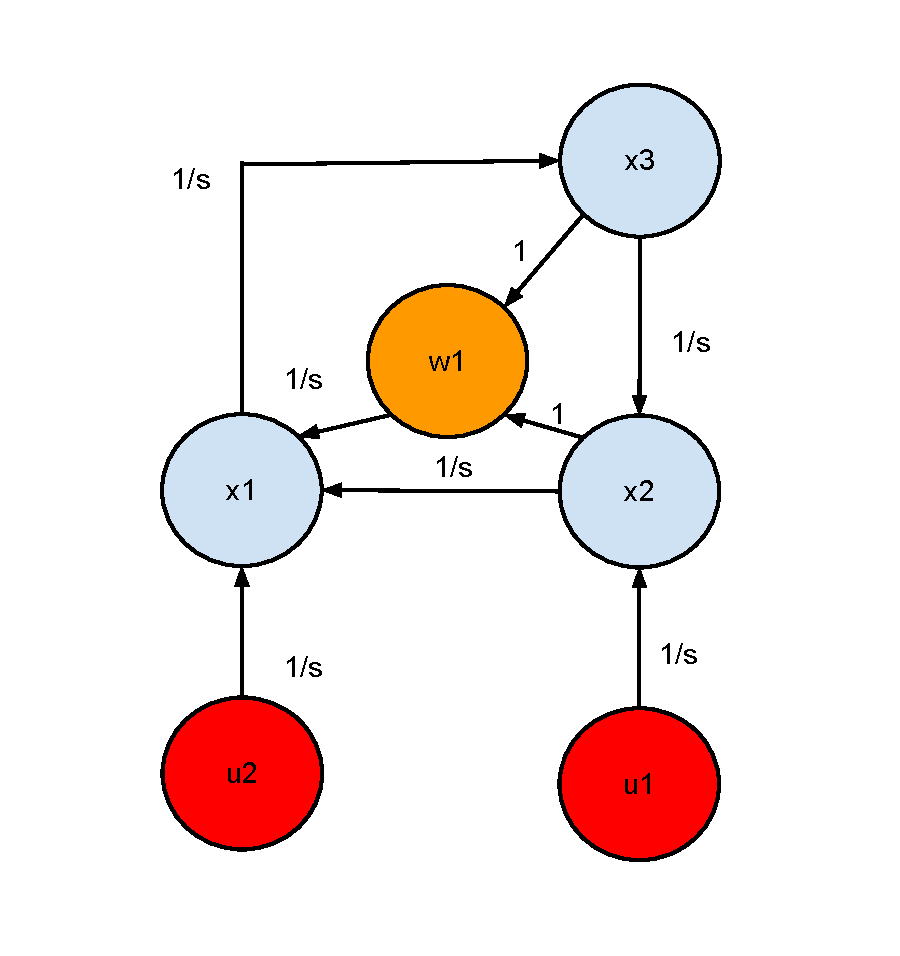
\includegraphics[scale=0.3,bb=0 0 153mm 162mm] {Figures/DAESFG.pdf}} 
\caption{SFG corresponding to the DAE in EQ. ~\ref{fig:eqDAE}.}
\label{fig:sfgDAE}
\end{figure}
%
The ODE-representation of the same system would become:
\begin{equation}\left[ \begin{array}{c} \dot{x_1} \\ \dot{x_2} \\ \dot{x_3} \end{array} \right]
= \begin{bmatrix} 0 & 2 & 1 \\ 0 & 0 & 1 \\ 1 & 0 & 0 \end{bmatrix} \left[ \begin{array}{c} x_1 \\ x_2 \\ x_3 \end{array} \right] + \begin{bmatrix} 0 & 1 \\ 1 & 0 \\ 0 & 0 \end{bmatrix}  \left[ \begin{array}{c} u_1 \\ u_2 \end{array} \right]
\label{fig:eqODEett}
\end{equation}
\begin{equation}\left[ \begin{array}{c} w_1  \end{array} \right]
=  \begin{bmatrix} 0 & 1 & 1\end{bmatrix} \left[ \begin{array}{c} x_1 \\ x_2 \\ x_3 \end{array} \right] + \begin{bmatrix} 0 & 0 \end{bmatrix}  \left[ \begin{array}{c} u_1 \\ u_2 \end{array} \right]
\label{fig:eqODE}
\end{equation}
\begin{figure}
\fbox{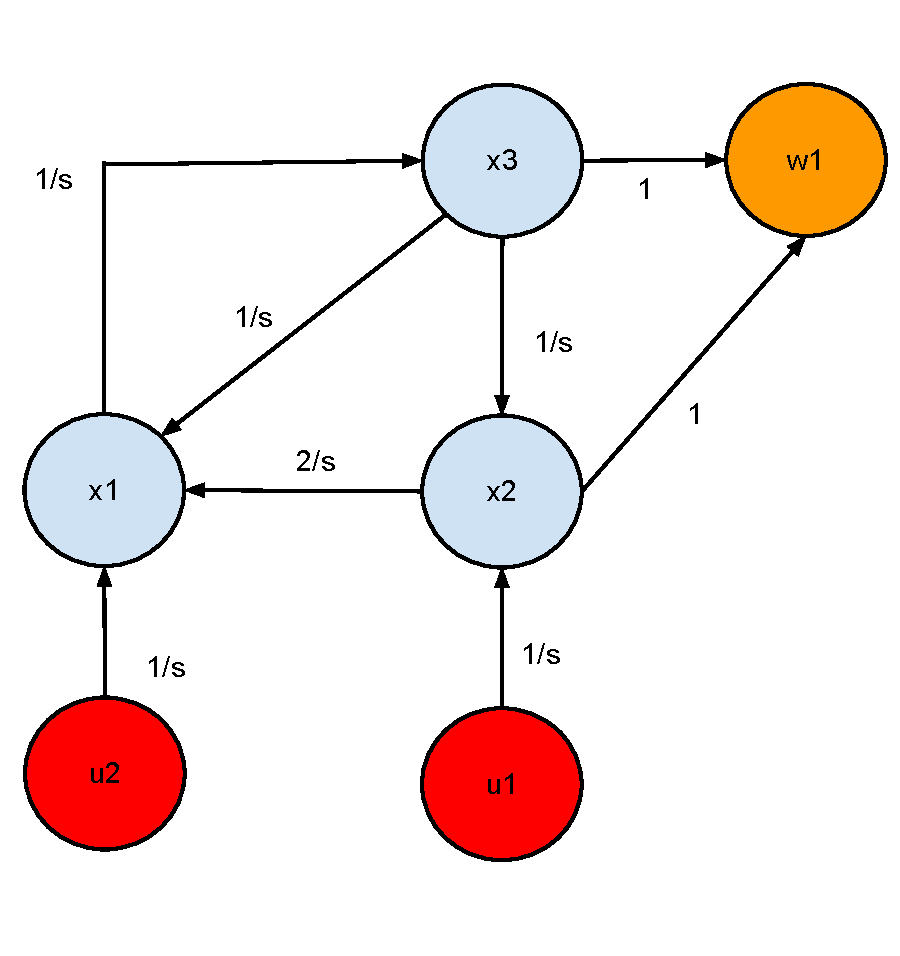
\includegraphics[scale=0.3,bb=0 0 153mm 162mm] {Figures/ODESFG.pdf}}
\caption{SFG corresponding to the ODE in EQ. ~\ref{fig:eqODEett} and EQ. ~\ref{fig:eqODE}.}
\label{fig:sfgODE}
\end{figure}%
As we can see, when comparing the SFG's in Fig. \ref{fig:sfgDAE} and Fig. \ref{fig:sfgODE}, the SFG-representations of the two systems will differ, we no longer can see the relation between $x_1$ and $w_1$. This is a problem since a user might want to analyse the relation between the algebraic variable and other points in the system directly.


%%==================================================================
%% Include bibliography references here
%% Replace the "thesisreferences" with your
%% own reference database
%%==================================================================
\bibliographystyle{ieeetr}

\fancyhead[LO]{}%
\fancyhead[RE]{}%
\fancyhead[LE]{\thepage}%
\fancyhead[RO]{\thepage}
\bibliography{thesisreferences}

\end{document}
